%! Author = abenjeddou
%! Date = 30/06/2026

\section{Introduction}
This chapter covers the sixth and final sprint, focused on implementing comprehensive observability through structured logging (Kibana), real-time metrics dashboards (Grafana), and alerting rules to ensure production-grade monitoring.

\section{Sprint Goal}

Our aim in this sprint is to implement comprehensive observability through structured logging (Kibana), real-time metrics dashboards (Grafana), and alerting rules to ensure production-grade monitoring.
\section{Job Visualization}

Figure~\ref{fig:flink-ui} illustrates the Flink user interface. In this view, we can observe elements such as the current job state and the available Task Managers for deploying the different tasks. This interface provides real-time visibility into the operation of our deployed Flink job, thus facilitating monitoring and troubleshooting.

\begin{center}
    \centering
    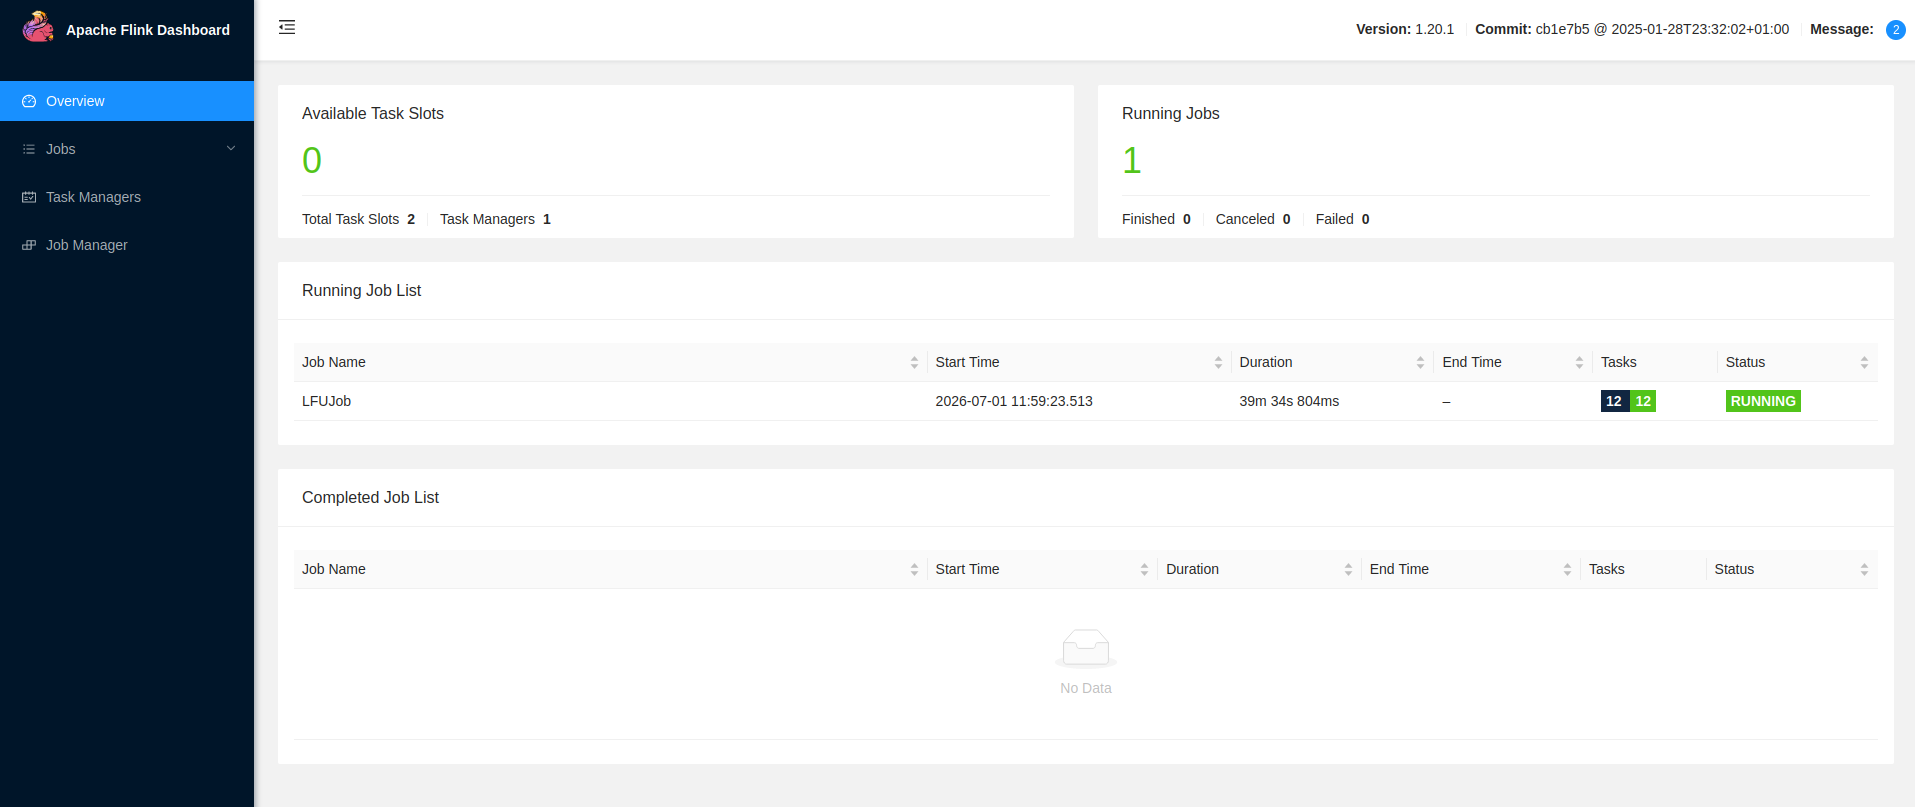
\includegraphics[width=1\textwidth]{img/flink_ui}
    \captionof{figure}{Flink user interface}
    \label{fig:flink-ui}
\end{center}

Figure~\ref{fig:flink-topology} represents the Flink job topology as well as an overview of the different deployed operators.
This illustrates how the different job components interact with each other to process data. More specifically, it shows the data path through the different operations of our job, from the initial source to the final destination.

\begin{center}
    \centering
    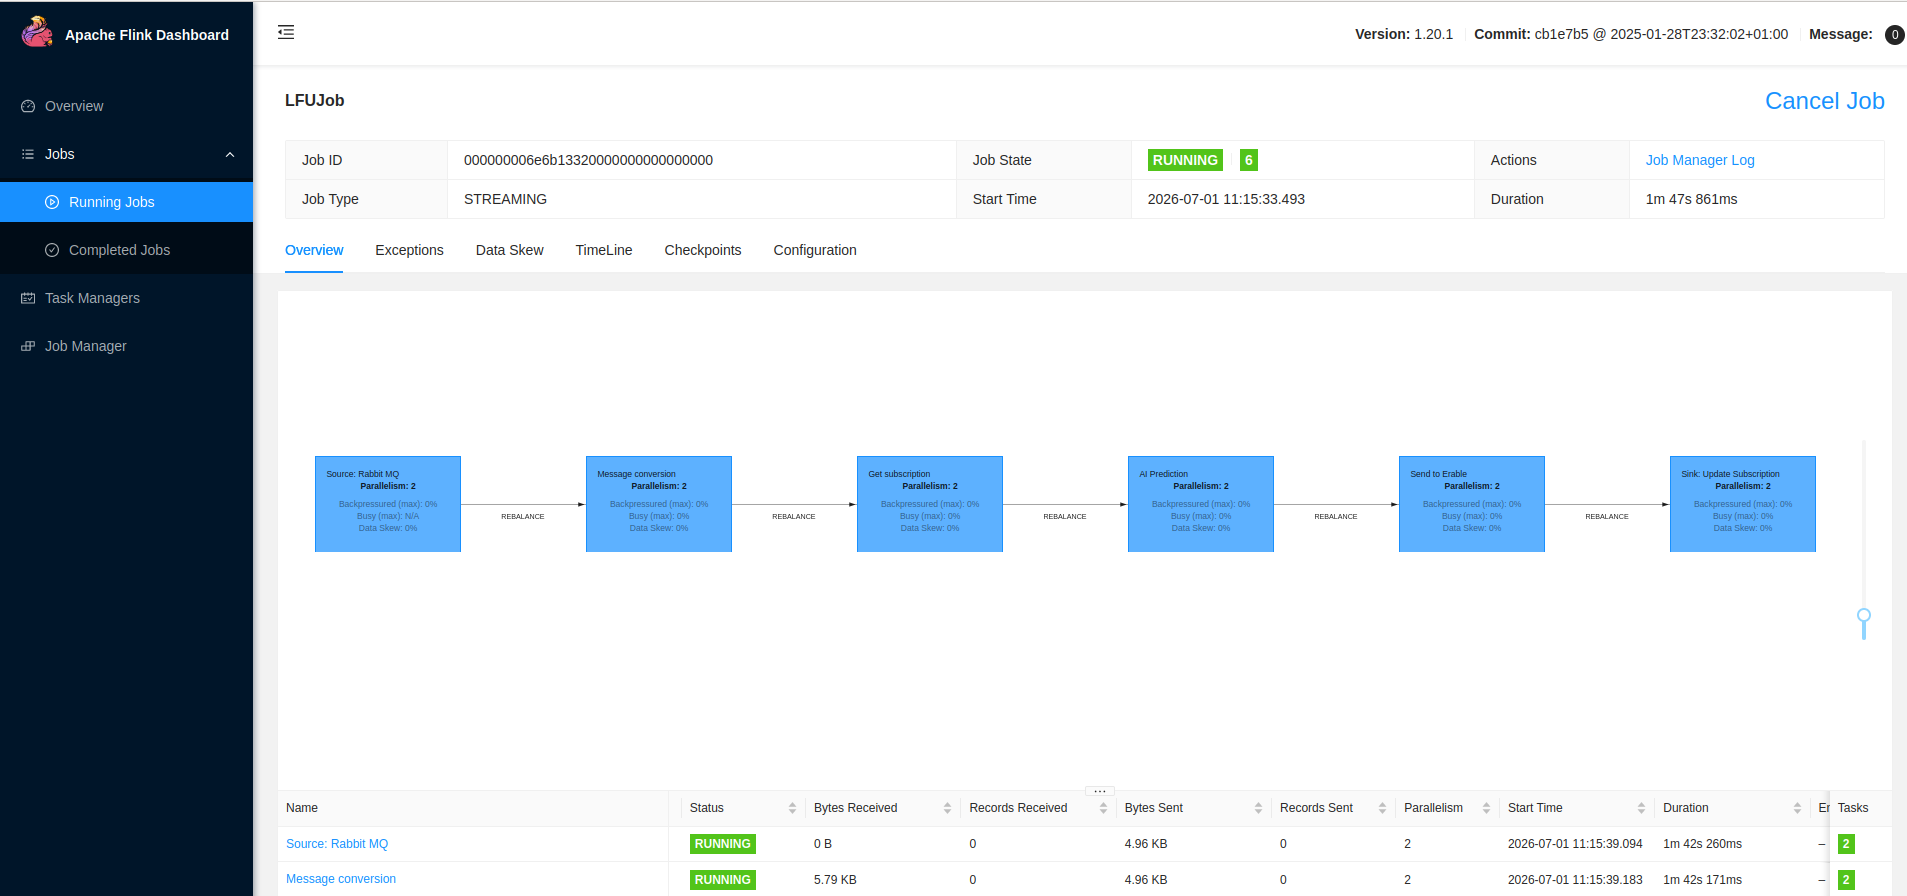
\includegraphics[width=1\textwidth]{img/flink_topology}
    \captionof{figure}{Job topology}
    \label{fig:flink-topology}
\end{center}

Figure~\ref{fig:flink-checkpoint} shows the checkpoints overview in the Flink UI. Here we can observe key checkpoint metrics such as the number of completed and failed checkpoints as well as the latest checkpoint duration and size.
It allows us to monitor the health of our state persistence mechanism and quickly identify any checkpoint failures or performance degradation that could compromise fault tolerance.

\begin{center}
    \centering
    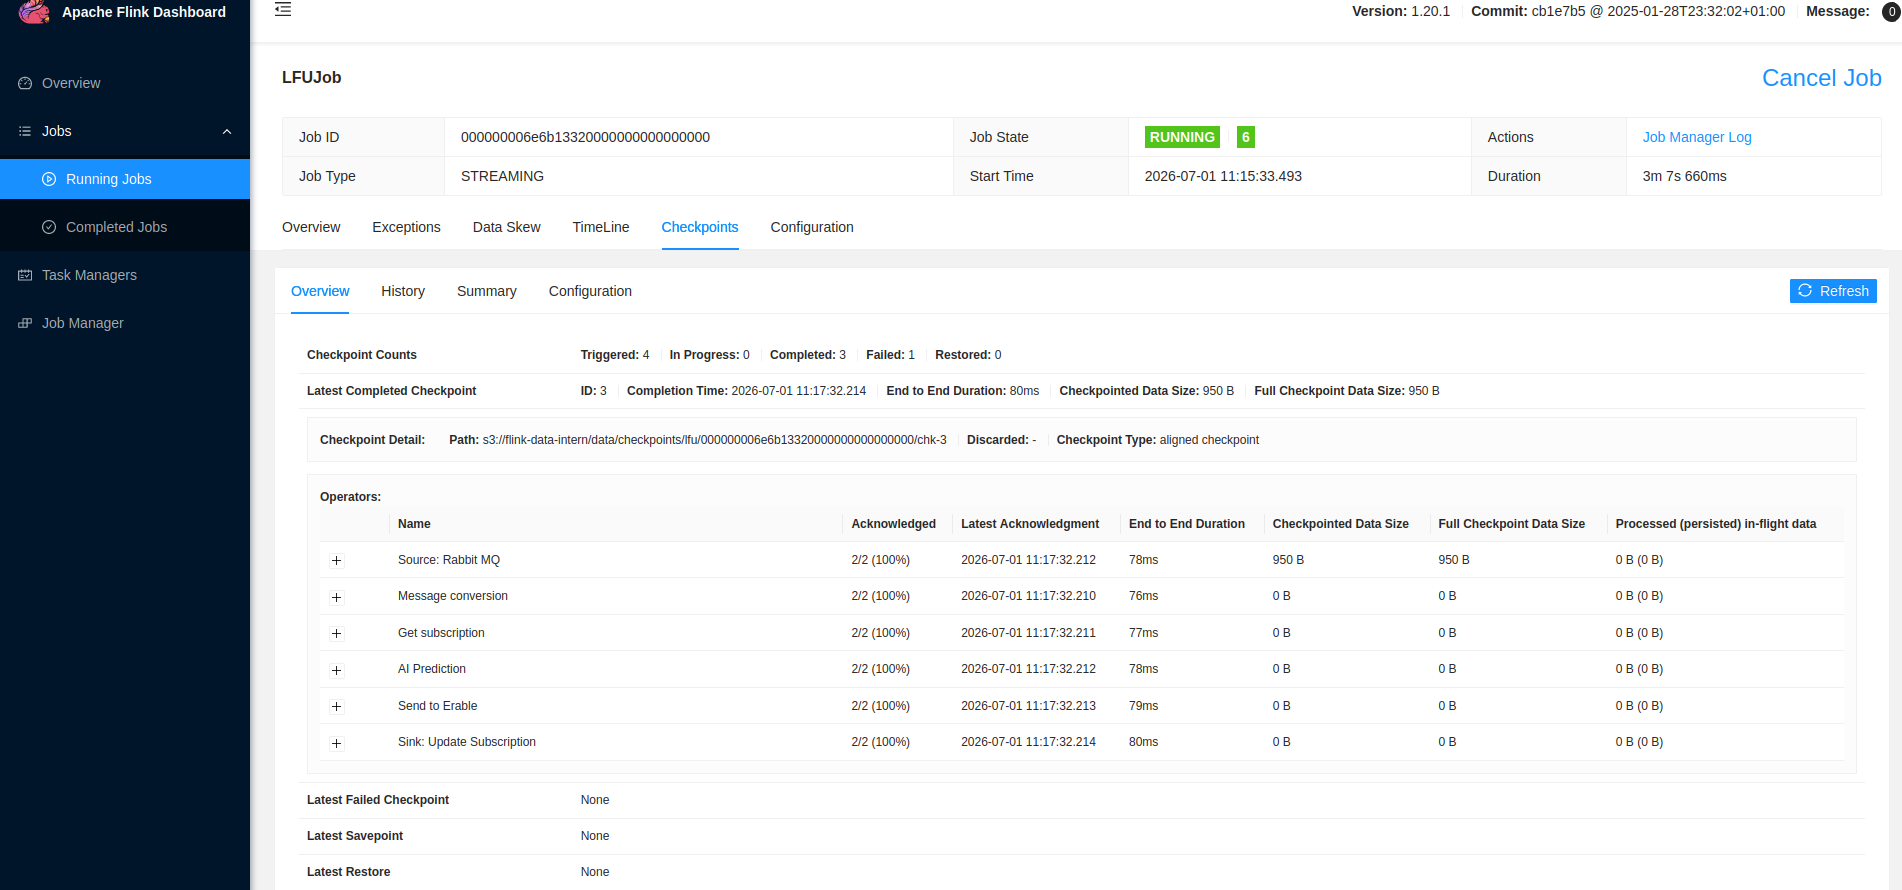
\includegraphics[width=1\textwidth]{img/checkpoint overview UI flink}
    \captionof{figure}{Checkpoint metrics overview}
    \label{fig:flink-checkpoint}
\end{center}

\section{Structured Logging}

\subsection{Log Architecture}

All log entries are structured as JSON using the \texttt{Logstash Logback Encoder}, enabling machine-parseable logs that are ingested into an \textbf{ELK stack}~\cite{elk} (Elasticsearch, Logstash, Kibana). Each log entry contains structured markers via \texttt{net.logstash.logback.marker.Markers.appendEntries()}.

Syslog sends logs to Logstash, which subsequently stores them in Elasticsearch.
They then become accessible for exploitation in the Kibana dashboard, enabling in-depth analyses and relevant visualizations.

\subsection{Log Keys}

Every log entry is enriched with the following structured fields, defined in \texttt{LogKeys}:

\begin{center}
    \begin{tabularx}{\textwidth}{|l|l|X|}
\toprule
\textbf{Field} & \textbf{Key} & \textbf{Description} \\
\midrule
\texttt{customCode} & \texttt{customCode} & Numeric code identifying the log event category (see Table~\ref{tab:log-codes}) \\ \hline
\texttt{uuid} & \texttt{uuid} & Unique message traceability identifier \\ \hline
\texttt{topologyName} & \texttt{topologyName} & Job name (\texttt{LFU}) \\ \hline
\texttt{sid} & \texttt{sid} & Service ID (OMOI, SOSH, OPRO) \\ \hline
\texttt{msisdn} & \texttt{msisdn} & Customer phone number \\ \hline
\texttt{X-ERABLE-uuid} & \texttt{X-ERABLE-uuid} & Erable request correlation UUID \\
\bottomrule
    \end{tabularx}
    \captionof{table}{Structured log fields}
    \label{tab:log-keys}
\end{center}

\subsection{Log Code Classification}

The \texttt{CodeMessageLog} enum provides a standardized classification for all log events:

\begin{center}
    \begin{tabularx}{\textwidth}{|l|l|l|X|}
\toprule
\textbf{Code} & \textbf{Level} & \textbf{Constant} & \textbf{Message} \\
\midrule
\multicolumn{4}{|l|}{\textit{Informational (0xxx--1xxx)}} \\
\hline
0000 & DEBUG & \texttt{INFORMATIONAL\_MESSAGE} & Informational message \\ \hline
1000 & INFO & \texttt{NOTIFICATION\_PROCESS\_COMPLETED} & Notification process completed \\
\midrule
\multicolumn{4}{|l|}{\textit{Success (2xxx)}} \\
\hline
2000 & DEBUG & \texttt{ERABLE\_SEND\_SUCCESSFULLY} & Notification sent to Erable successfully \\
\midrule
\multicolumn{4}{|l|}{\textit{Discarded (2xxx)}} \\
\hline
2041 & INFO & \texttt{NOTIFICATION\_DISCARDED} & Notification discarded \\ \hline
2045 & WARN & \texttt{UNMANAGED\_EVENT} & Unmanaged event type for notif \\ \hline
2047 & INFO & \texttt{NO\_MAIN\_RECORD\_FOR\_NOTIF} & No main record for notif \\
\midrule
\multicolumn{4}{|l|}{\textit{Client Errors (4xxx)}} \\
\hline
4000 & ERROR & \texttt{MISSING\_MANDATORY\_PARAMETERS} & Missing mandatory parameters \\ \hline
4150 & ERROR & \texttt{NOT\_VALID\_JSON} & Not valid JSON \\ \hline
4401 & ERROR & \texttt{NO\_DATA} & No data \\
\midrule
\multicolumn{4}{|l|}{\textit{System Errors (5xxx)}} \\
\hline
5030 & ERROR & \texttt{ERABLE\_ACCESS\_ERROR} & Erable access error \\ \hline
5031 & ERROR & \texttt{PERSISTENCE\_LIB\_ACCESS\_ERROR} & Valkey access error \\ \hline
5036 & ERROR & \texttt{UNMANAGED\_ERROR} & Unmanaged error \\
\bottomrule
    \end{tabularx}
    \captionof{table}{Log code classification (\texttt{CodeMessageLog})}
    \label{tab:log-codes}
\end{center}

\subsection{Log Example}

A typical structured log entry produced by the LFU job:

\begin{lstlisting}[caption={Structured JSON log entry example}]
{
  "timestamp": "2026-06-30T14:32:15.123+02:00",
  "level": "INFO",
  "logger": "LFUGetSubscriptionProcessFunction",
  "message": "Processing notification, main record found",
  "customCode": "0000",
  "uuid": "a1b2c3d4-e5f6-7890-abcd-ef1234567890",
  "topologyName": "LFU",
  "sid": "omoi",
  "msisdn": "33612345678"
}
\end{lstlisting}

\section{Kibana Dashboards}

The structured logs are ingested into Elasticsearch and visualized through Kibana dashboards. Thanks to Kibana, we have the ability to access the logs of our Flink job, offering the capability to filter data or generate precise statistics over well-defined time periods.

Key Kibana queries used for monitoring:

\begin{center}
    \begin{tabularx}{\textwidth}{|l|X|}
\toprule
\textbf{Purpose} & \textbf{KQL Query} \\
\midrule
All LFU logs & \texttt{topologyName:"LFU"} \\ \hline
Errors only & \texttt{topologyName:"LFU" AND level:"ERROR"} \\ \hline
Erable failures & \texttt{topologyName:"LFU" AND customCode:"5030"} \\ \hline
Valkey failures & \texttt{topologyName:"LFU" AND customCode:"5031"} \\ \hline
Discarded messages & \texttt{topologyName:"LFU" AND customCode:"2041"} \\ \hline
Successful deliveries & \texttt{topologyName:"LFU" AND customCode:"2000"} \\ \hline
Completed notifications & \texttt{topologyName:"LFU" AND customCode:"1000"} \\ \hline
Track specific customer & \texttt{topologyName:"LFU" AND msisdn:"33612345678"} \\ \hline
Trace by UUID & \texttt{uuid:"a1b2c3d4-..."} \\ \hline
AI anomalies & \texttt{topologyName:"LFU" AND message:"Anomaly detected"} \\
\bottomrule
    \end{tabularx}
    \captionof{table}{Kibana queries for LFU monitoring}
    \label{tab:kibana-queries}
\end{center}


Figure~\ref{fig:log-subscription-found} shows a Kibana log entry corresponding to a successful subscription retrieval. We can observe the structured fields such as the \texttt{topologyName}, \texttt{msisdn}, and \texttt{customCode} indicating that the main record was found for the customer, allowing the pipeline to proceed with notification processing.

\begin{center}
    \centering
    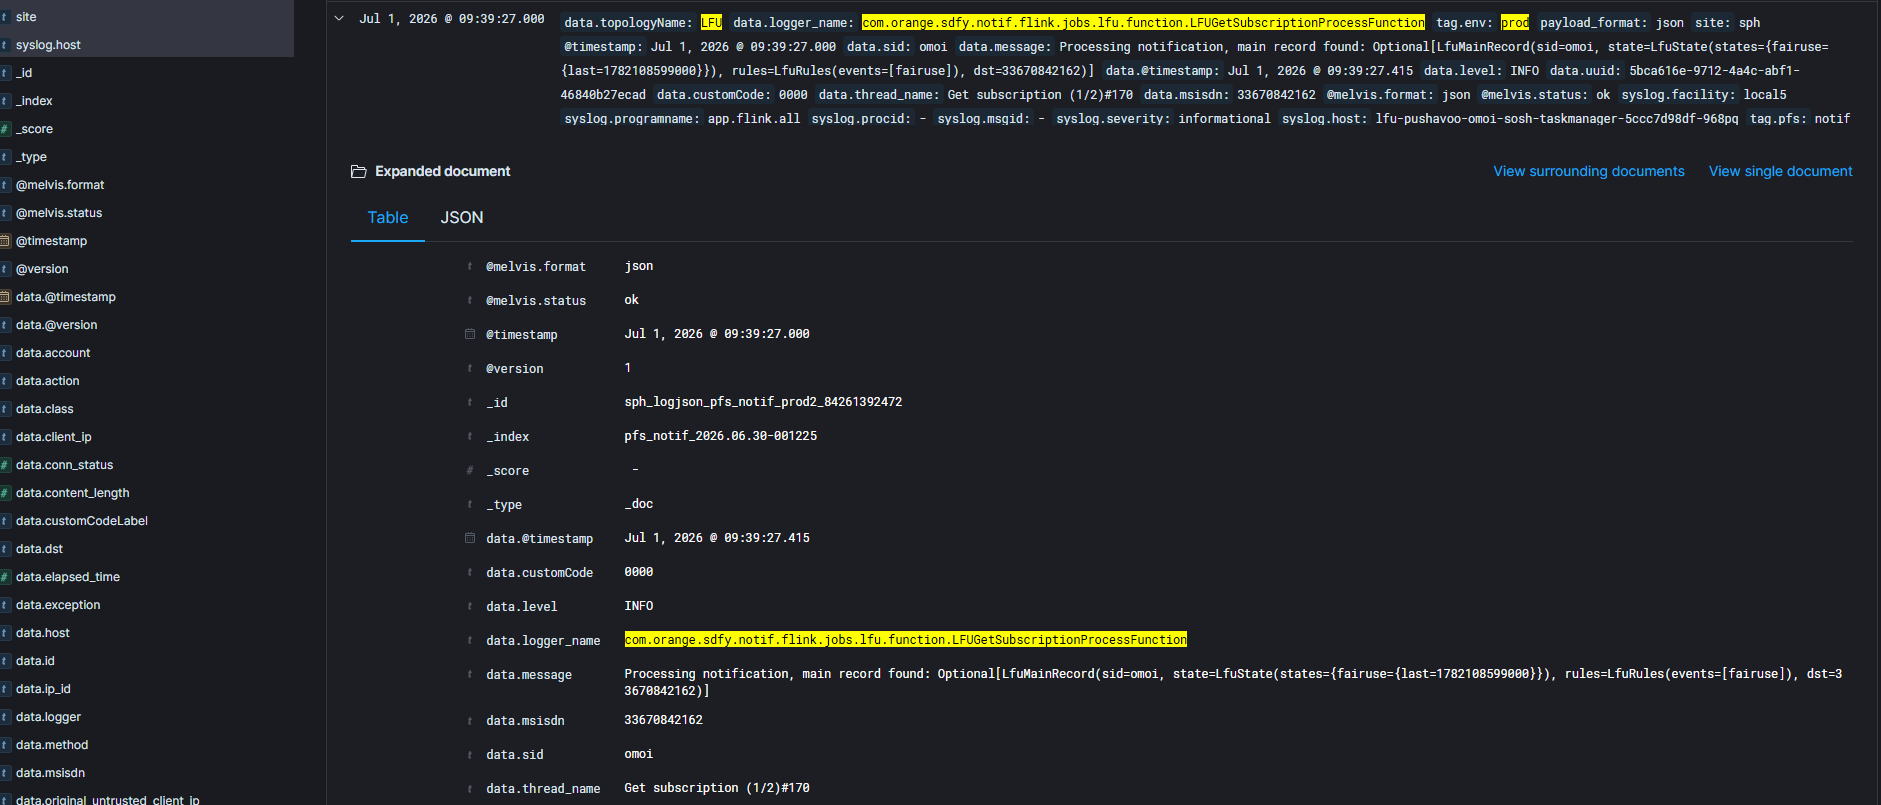
\includegraphics[width=1\textwidth]{img/subscription found log}
    \captionof{figure}{Kibana log entry: subscription found}
    \label{fig:log-subscription-found}
\end{center}

Figure~\ref{fig:log-erable-problem} illustrates a Kibana log entry showing an Erable access error (code 5030). This type of log appears when the Flink job fails to reach the Erable API for notification dispatching. The structured log format enables the admin to quickly filter all occurrences of this error and correlate them with potential network outages or API unavailability.

\begin{center}
    \centering
    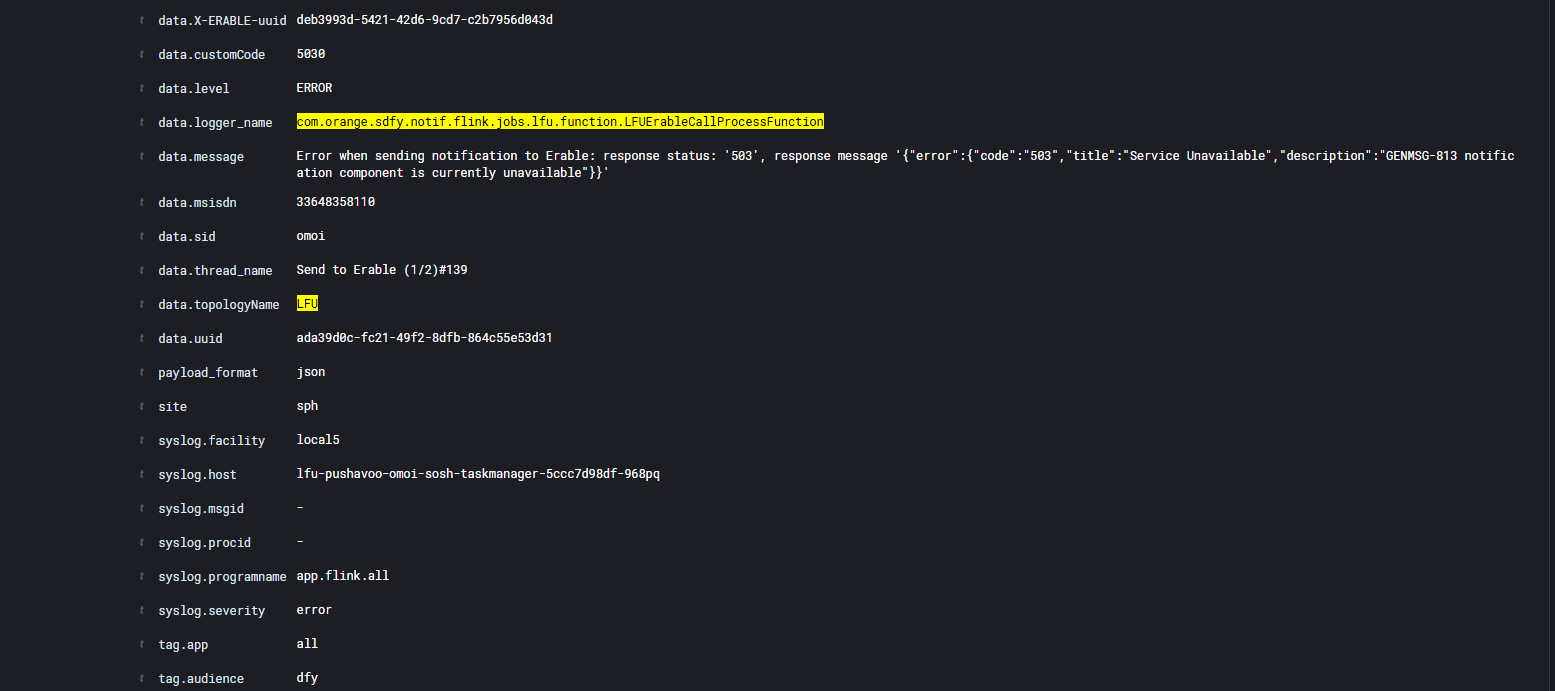
\includegraphics[width=1\textwidth]{img/Erable problem log}
    \captionof{figure}{Kibana log entry: Erable access error (5030)}
    \label{fig:log-erable-problem}
\end{center}

Figure~\ref{fig:log-anomaly-detected} shows a Kibana log entry produced by the AI module when a consumption anomaly is detected. The structured log includes the anomaly message emitted when the predicted score exceeds the configured threshold. This allows the admin to quickly filter all anomaly events and monitor unusual consumption patterns flagged by the model.

\begin{center}
    \centering
    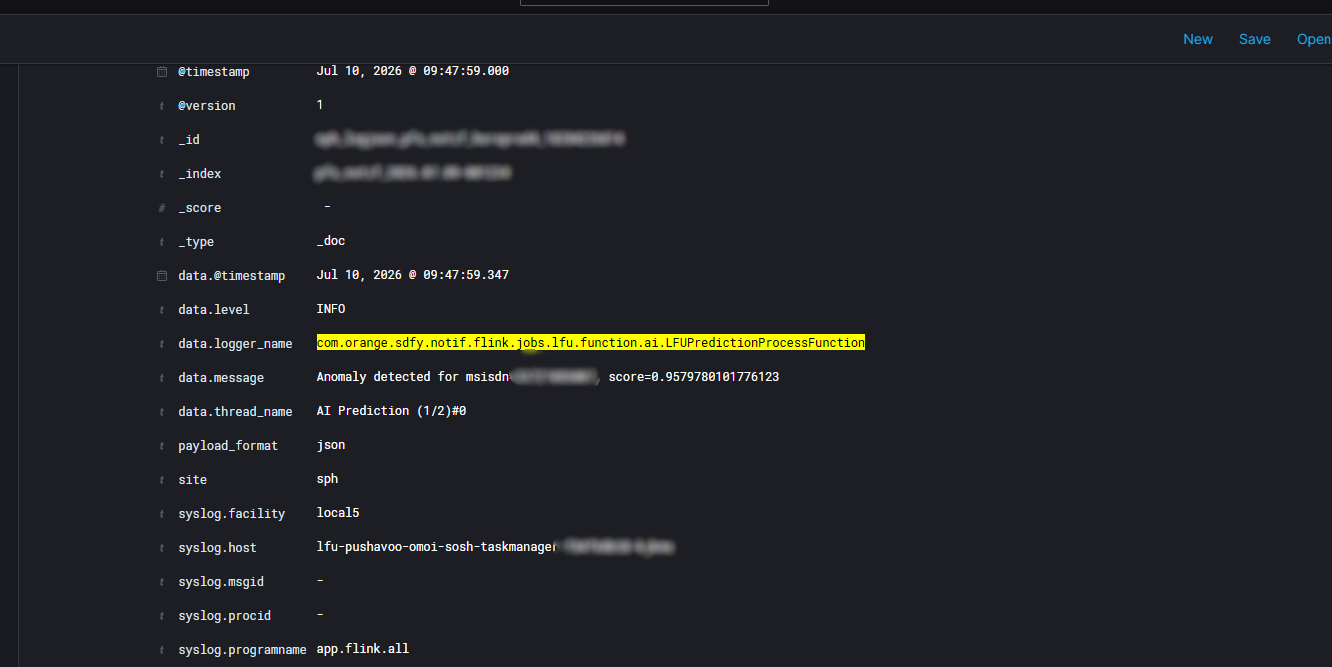
\includegraphics[width=1\textwidth]{img/anomaly kibana}
    \captionof{figure}{Kibana log entry: AI anomaly detected}
    \label{fig:log-anomaly-detected}
\end{center}



\section{Flink Metrics}

Each operator exposes counters via the Flink metrics system. These are scraped by \textbf{Prometheus}~\cite{prometheus} (port 9249) and visualized in \textbf{Grafana}~\cite{grafana}.

Prometheus~\cite{prometheus} operates on the scraping model, regularly querying the job endpoint exposing metrics (/metrics). Grafana~\cite{grafana} is a visualization and dashboard platform that connects to various data sources, including Prometheus, displaying data in the form of interactive and customizable dashboards.

\begin{center}
    \begin{tabularx}{\textwidth}{|l|l|X|}
\toprule
\textbf{Metric} & \textbf{Operator} & \textbf{Description} \\
\midrule
\texttt{incoming\_requests} & Validation & Total number of messages received \\ \hline
\texttt{discarded\_requests} & Validation, Subscription & Messages rejected (invalid or no main record) \\ \hline
\texttt{failed\_requests} & Subscription, Erable, Sink & Valkey or Erable access errors \\ \hline
\texttt{sent\_requests\_omoi} & Erable & Notifications sent for Orange et Moi \\ \hline
\texttt{sent\_requests\_sosh} & Erable & Notifications sent for My Sosh \\ \hline
\texttt{sent\_requests\_opro} & Erable & Notifications sent for Orange Pro \\ \hline
\texttt{predictions\_total} & AI & Total number of predictions performed \\ \hline
\texttt{anomalies\_detected} & AI & Consumption anomalies detected \\ \hline
\texttt{fallback\_used} & AI & Predictions using rule-based fallback \\
\bottomrule
    \end{tabularx}
    \captionof{table}{Metrics exposed by the LFU job}
    \label{tab:runtime-metrics}
\end{center}

\section{Grafana Dashboards}

Four Grafana dashboards were created for comprehensive LFU monitoring.

\subsection{Dashboard 1: Job Overview and QoS}

Figure~\ref{fig:grafana-1} presents the first Grafana dashboard, which provides an overview of the running job's health. It displays key indicators such as the current job status, the number of restarts, and Quality of Service (QoS) metrics. This dashboard allows operators to quickly assess whether the job is running normally or if unexpected restarts have occurred, which could indicate stability issues.

\begin{center}
    \centering
    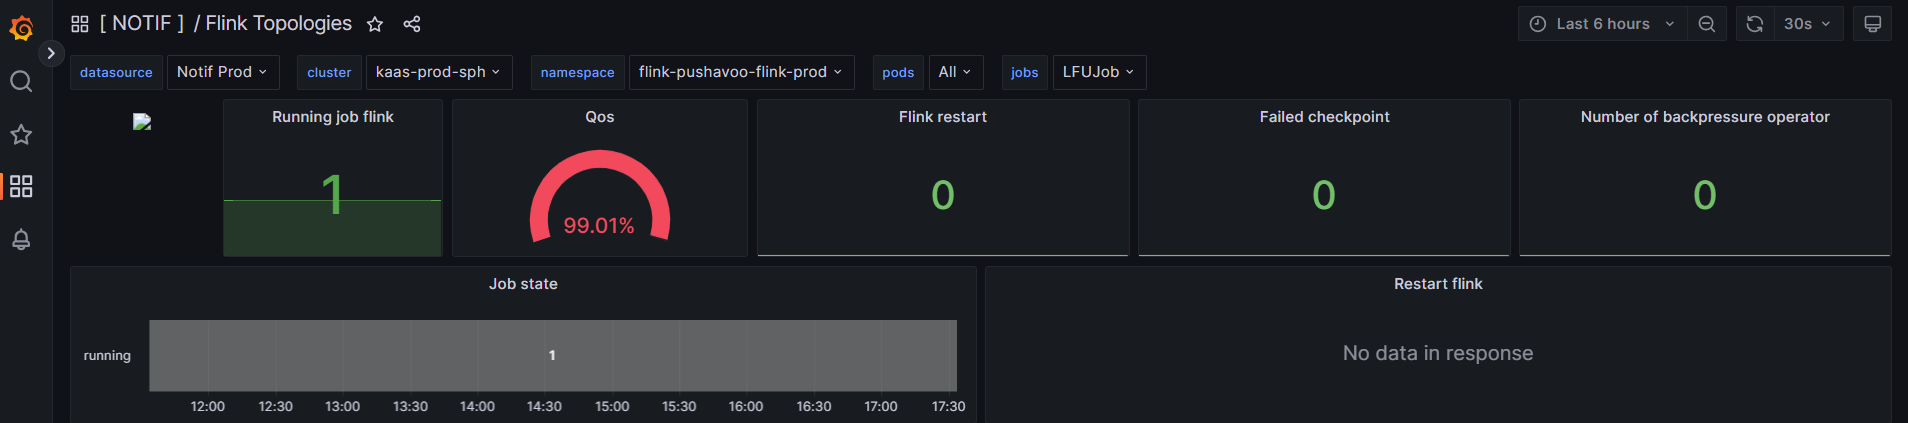
\includegraphics[width=1\textwidth]{img/lfu grafana 1}
    \captionof{figure}{Grafana dashboard: Job overview and QoS}
    \label{fig:grafana-1}
\end{center}

\subsection{Dashboard 2: Event Metrics}

Figure~\ref{fig:grafana-2} shows the second Grafana dashboard, focused on event-level metrics. It tracks the number of events sent, discarded, and errored over time. This dashboard provides a clear picture of the pipeline's throughput and error rates, enabling operators to detect anomalies in message processing patterns and identify potential issues with downstream services.

\begin{center}
    \centering
    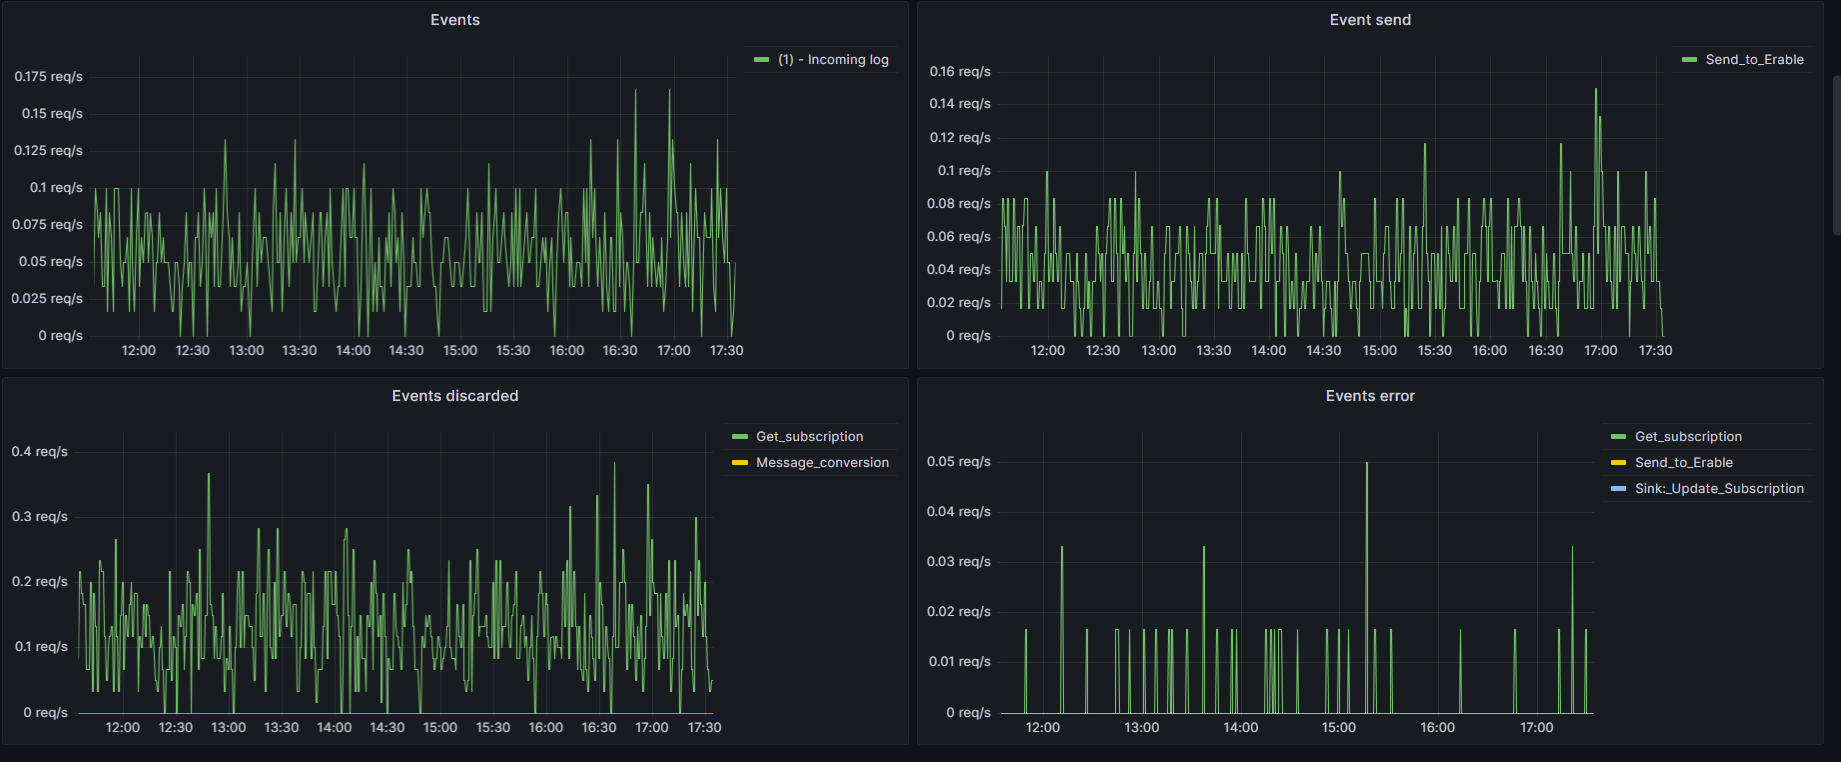
\includegraphics[width=1\textwidth]{img/lfu grafana 2}
    \captionof{figure}{Grafana dashboard: Event metrics}
    \label{fig:grafana-2}
\end{center}

\subsection{Dashboard 3: Resource Monitoring}

Figure~\ref{fig:grafana-resources} displays the resource monitoring dashboard, which tracks CPU usage, memory consumption, and system load across the Flink cluster. This dashboard is essential for capacity planning and detecting resource bottlenecks. It allows operators to monitor whether TaskManagers are approaching their resource limits and to anticipate scaling needs.

\begin{center}
    \centering
    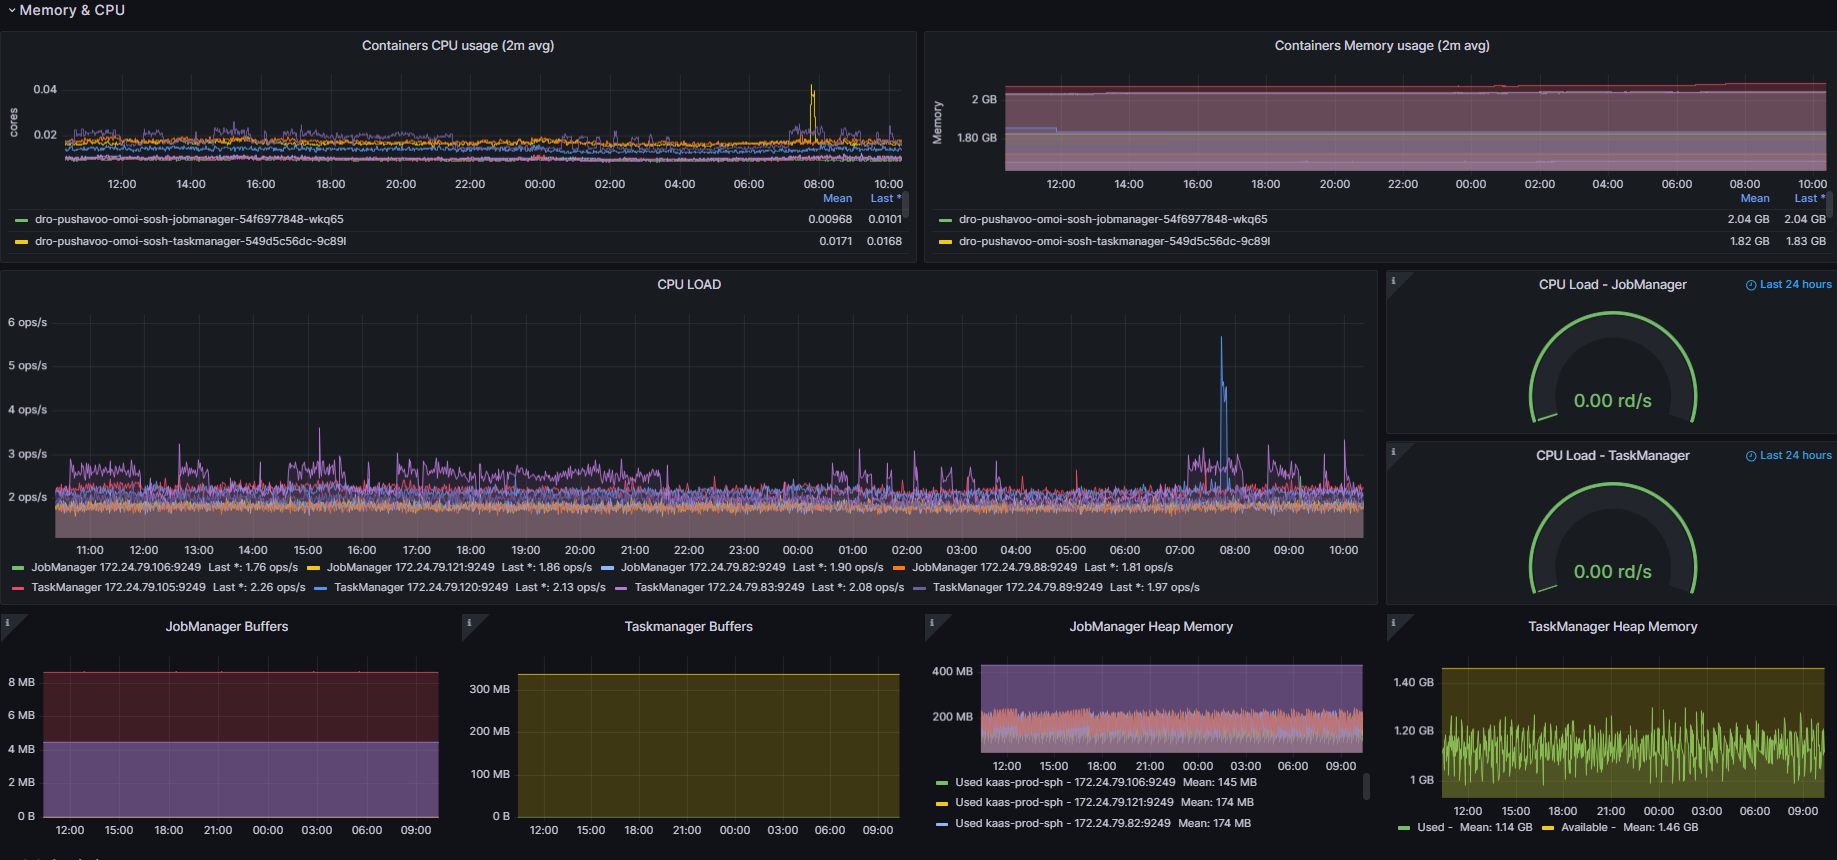
\includegraphics[width=1\textwidth]{img/grafana for resources}
    \captionof{figure}{Grafana dashboard: Resource monitoring}
    \label{fig:grafana-resources}
\end{center}

\subsection{Dashboard 4: Job Statistics}

Figure~\ref{fig:grafana-job-stats} presents the job statistics dashboard, which provides detailed metrics on records flowing through the pipeline --- specifically records in and records out per operator. This dashboard enables operators to identify processing bottlenecks, verify data flow consistency, and ensure that no records are silently lost between operators.

\begin{center}
    \centering
    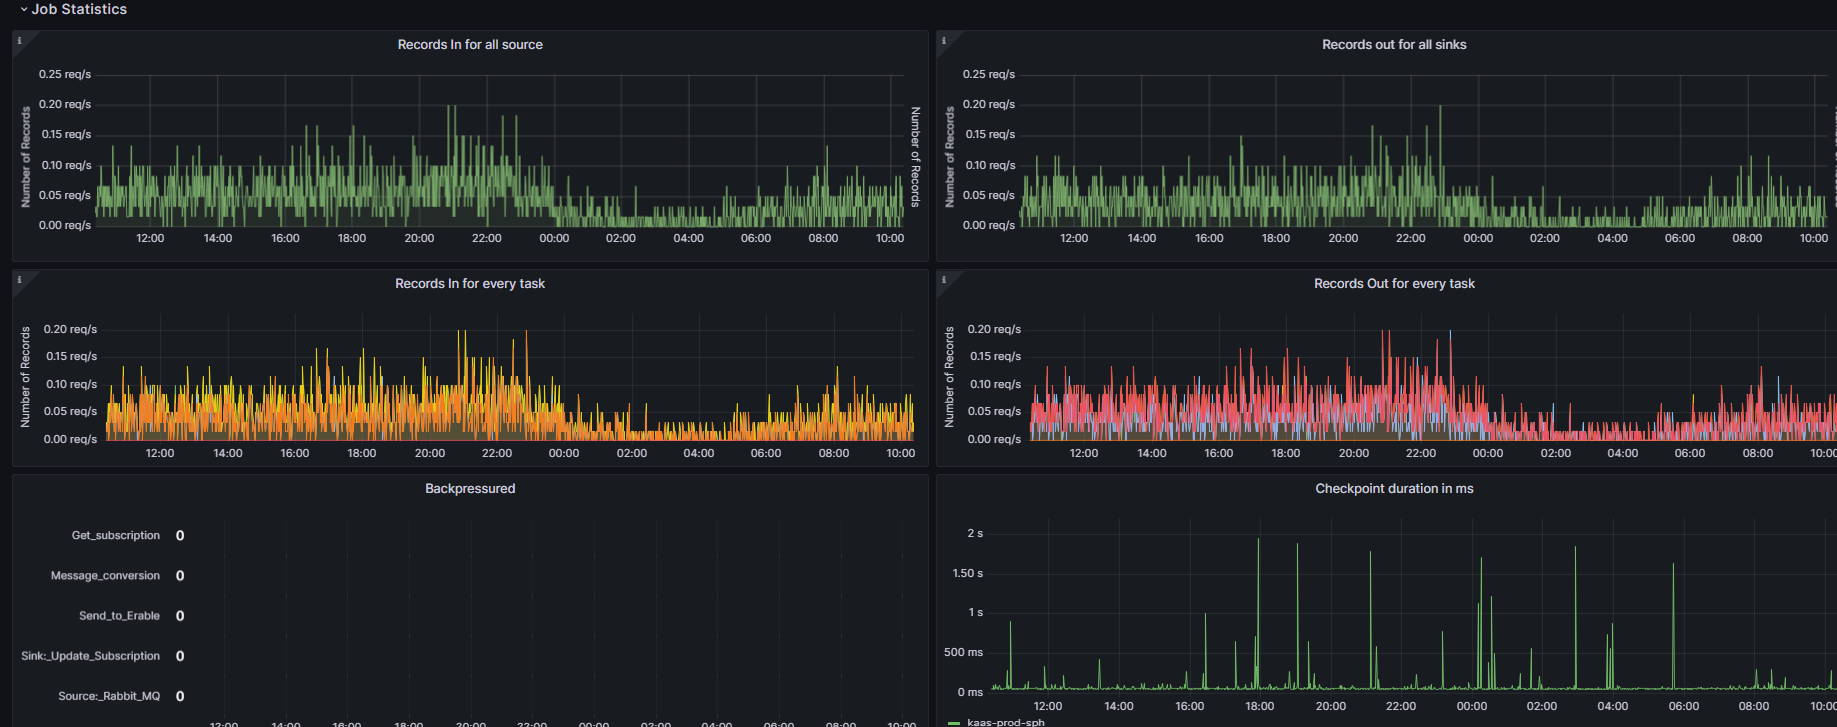
\includegraphics[width=1\textwidth]{img/grafana for job stats}
    \captionof{figure}{Grafana dashboard: Job statistics}
    \label{fig:grafana-job-stats}
\end{center}

\section{Alerting Rules}

The following Prometheus alerting rules are configured to trigger PagerDuty/email notifications:

\begin{center}
    \begin{tabularx}{\textwidth}{|l|l|X|}
\toprule
\textbf{Alert Name} & \textbf{Condition} & \textbf{Description} \\
\midrule
\texttt{LFUHighErrorRate} & Error ratio $> 5\%$ for 5~min & Too many messages failing \\ \hline
\texttt{LFUErableDown} & Erable failures $> 10$/min for 5~min & Erable API unreachable \\ \hline
\texttt{LFUValkeyDown} & Valkey failures $> 10$/min for 5~min & Valkey state store unreachable \\ \hline
\texttt{LFUAIFallbackActive} & \texttt{fallback\_used} $> 0$ for 10~min & ONNX model not loaded \\ \hline
\texttt{LFUHighAnomalyRate} & Anomaly ratio $> 20\%$ for 15~min & Unusual consumption patterns \\ \hline
\texttt{LFUNoIncoming} & \texttt{incoming\_requests} $= 0$ for 10~min & No messages received \\ \hline
\texttt{LFUCheckpointFailing} & Checkpoint failures $> 3$ & State consistency at risk \\
\bottomrule
    \end{tabularx}
    \captionof{table}{Prometheus alerting rules}
    \label{tab:alerts}
\end{center}

\section{End-to-End Traceability}

A single notification can be traced through the entire system using the \texttt{uuid} field:

\begin{enumerate}
    \item \textbf{Kibana}: Search by \texttt{uuid} to see every log entry for a specific message, from ingestion through delivery.
    \item \textbf{Grafana}: Correlate timestamps from Kibana with metric spikes (e.g., an error burst at 14:32 matching an Erable outage).
    \item \textbf{Erable}: The \texttt{X-ERABLE-uuid} field allows tracing the notification into the downstream push notification system.
\end{enumerate}

\section{Testing}

The job is covered across all sprints by:
\begin{itemize}
    \item \textbf{Unit tests using JUNIT~\cite{junit}}: Each operator is tested in isolation with mocks (Mockito 4.5.1) for Valkey and Erable. Log assertions validate that correct \texttt{CodeMessageLog} entries are emitted using the shared \texttt{LogAssertionUtils}.
    \item \textbf{Integration tests using JUNIT}: Full pipeline validation with a local Flink environment and mocked external services.
    \item \textbf{End-to-end tests using Jmeter~\cite{jmeter}}: Message publication to local RabbitMQ and verification of the Valkey state output.
\end{itemize}

The \texttt{pushavoo-flink-test} module provides shared test utilities across all jobs, including \texttt{LogAppender} for capturing and asserting structured log output.

\section*{Conclusion}

At the end of Sprint~6, the LFU job had complete production observability. Operators could monitor the system in real time through Grafana dashboards and investigate specific issues through Kibana log search. Alerting rules provided proactive notification of system degradation.

Over 6 sprints, the LFU job was developed incrementally from a simple message consumer to a fully observable, AI-enhanced notification pipeline. This architecture enables the processing of fair-use events with minimal latency while guaranteeing the reliability of the push notification system for millions of Orange customers.

